\chapter{Puesta a prueba de la DAQ + Lock-in Digital} 
\label{apéndice:prueba_lockin_digital} %  .   

% \missingfigure{Amplitud y fase RLC serie } 

Para verificar el correcto funcionamiento del lock-in digital implementado junto a la placa de adquisición se caracterizó la respuesta en frecuencia de un circuito bien determinado teórica y experimentalmente previamente. El elegido fue un RLC serie como con el que se trabajará para las mediciones de altura de superficie libre con el sensor. Los resultados obtenidos se muestran en la Figura \ref{fig:apendice}. 

\begin{figure}[th!] 
	\centering
	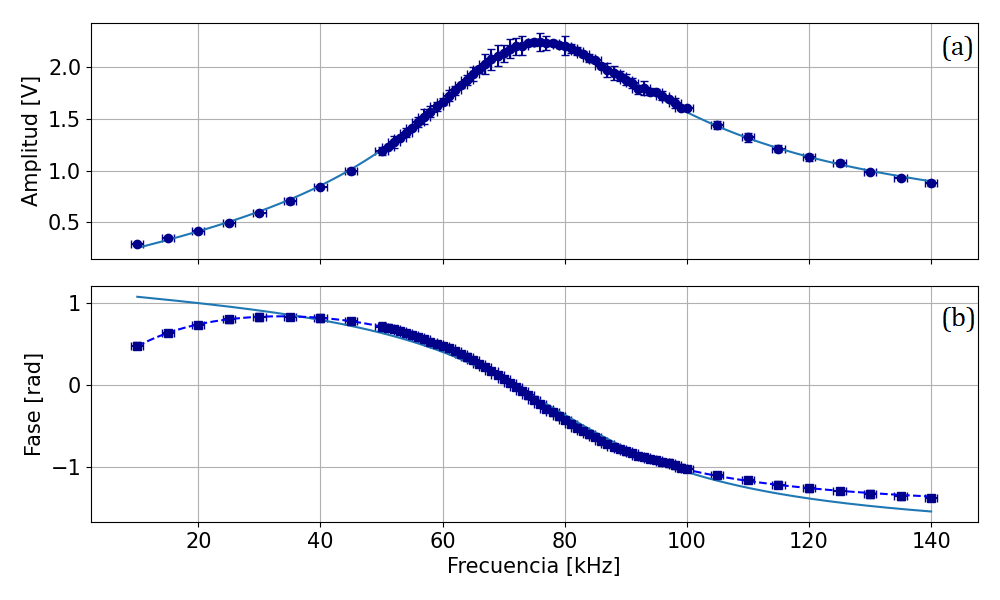
\includegraphics[width=0.987\linewidth]{Figuras/Sensor/Apéndice/Apéndice}
	\caption{Respuesta en frecuencia para una RLC serie (\markcircle*[blue]{0.4ex}) obtenida mediante la placa de adquisición y el algoritmo de lock-in digital (a) Amplitud y (b) Fase. Se muestran los ajustes por la respuesta teórica (\marksolid[blue]{0.4ex}) y en el caso de particular de la fase con una correción que tiene en cuenta una capacitancia parásita acoplada a modo de filtro pasa-altos (\markdashed[blue]{0.4ex}). } % . 
	\label{fig:apendice}
\end{figure} 


Aquí no interesan tantos los resultados para los parámetros obtenidos sino que los datos obtenidos se corresponden al modelo que se esperaría. Los valores obtenidos son los de la Tabla \ref{tab:rlc_fit_params}.  

\begin{table}[h!]
	\centering
	\begin{tabular}{ |c | c | c | c | c | }       
		\hline
		Ajuste & Parámetros & Valores ± Incertidumbre & $R^2$ & $\chi^2_\nu$ \\ 
		\hline
		Amplitud & $A_0$, $f_0$, $Q$, $B$ & $(2.125 \pm 0.0071)$, $(7.631\times 10^4 \pm 92)$, $(2.01 \pm 0.015)$, $(0.1304 \pm 0.0031)$ & 0.99864 & 2.239 \\
		Fase (sin corrección) & $Q$, $f_0$, $B$ & $(1.762 \pm 0.0016)$, $(7.996\times 10^4 \pm 1.3\times 10^2)$, $(-0.3251 \pm 0.0029)$ & 0.96429 & 70.375 \\
		Fase (corregida) & $Q$, $f_0$, $B$, $f_c$ & $(1.979 \pm 0.0067)$, $(7.627\times 10^4 \pm 1.1\times 10^2)$, $(-0.03815 \pm 0.007)$, $(1.548\times 10^4 \pm 4.4\times 10^2)$ & 0.99984 & 0.275 \\
		\hline 
	\end{tabular} 
	\caption{Parámetros obtenidos de los ajustes de amplitud y fase, incluyendo incertidumbres, $R^2$ y $\chi^2_\nu$.}
	\label{tab:rlc_fit_params}
\end{table}

Se concluye a partir de estos resultados el buen funcionamiento del lock-in digital y la placa de adquisición. 



